\documentclass{hitec}
\author{FOSSEE, IIT Bombay}
\title{A library for Hardware-In-Loop for OpenModelica}

\usepackage{forest}
\usepackage{graphicx}
\usepackage[T1]{fontenc}
\usepackage[utf8]{inputenc}
\usepackage{lmodern,hyperref,graphicx,tcolorbox,listings,fancyhdr,longtable,caption,color,dblfnote}
\usepackage[titletoc]{appendix}
\usepackage[english]{babel}

\begin{document}
\maketitle
\section{Introduction}
This document has been written with the intent of familiarising a user with the Modelica H-I-L toolbox developed at FOSSEE. The InterProcessCommunication package, which is central to this toolbox, was developed at ModeliCon with the intent of communicating between two PCs. The team at FOSSEE modified it to function with an Arduino Mega and a PC. 

The reason the IPC package was chosen over conventional packages is its ability to transfer data independent of data type. This comes in handy when dealing with the vast range of values that can be assumed while working with a controller such as a PID. 

\section{Directory Structure}
The directory structure for the library is described below. Also as package.mo and package.order are present in multiple directories within InterProcessCommunication, and are largely irrelevant to direct usage, only those at the top level have been listed.\\
\begin{forest}
  for tree={
    font=\ttfamily,
    grow'=0,
    child anchor=west,
    parent anchor=south,
    anchor=west,
    calign=first,
    edge path={
      \noexpand\path [draw, \forestoption{edge}]
      (!u.south west) +(7.5pt,0) |- node[fill,inner sep=1.25pt] {} (.child anchor)\forestoption{edge label};
    },
    before typesetting nodes={
      if n=1
        {insert before={[,phantom]}}
        {}
    },
    fit=band,
    before computing xy={l=15pt},
  }
[
  [ArduinoCode
    [ArduIPCWrite
    	[ArduIPCWrite.ino]]
    [basic\_ write
    	[basic\_ write.ino]]
    [IPC\_ PID
    	[IPC\_ PID.ino]]
  ]
  ]
  \end{forest}
  
  \begin{forest}
   for tree={
    font=\ttfamily,
    grow'=0,
    child anchor=west,
    parent anchor=south,
    anchor=west,
    calign=first,
    edge path={
      \noexpand\path [draw, \forestoption{edge}]
      (!u.south west) +(7.5pt,0) |- node[fill,inner sep=1.25pt] {} (.child anchor)\forestoption{edge label};
    },
    before typesetting nodes={
      if n=1
        {insert before={[,phantom]}}
        {}
    },
    fit=band,
    before computing xy={l=15pt},
  }
  [
  [InterProcessCommunication
    [Examples
    [CombinedExamples
    [PIDandMotor.mo]
    [PulsePIDandMotor.mo]
    	]
    [InterProcessExamples
    [ArduinoIPC.mo]
    [DC\_ Motor\_ Arduino.mo]
    	]
    	]
    [Info
    [Tutorial
	[Advanced.mo]
	[GettingStarted.mo]    
    	]
    [Contact.mo]
    [Overview.mo]
        	]
    [Resources
    [Include
    [Arduino\_ port.sh]
    [SerialMI.h]
    [Serial\_ SHM.c]
    [ShmMI.c]	]
    [Library
    [linux64
    [librt.a]
    [librt.so]
    	]	
    	]
    	]
    [SharedMemory
    [SharedMemoryRead.mo]
    [SharedMemoryWrite.mo]]
    [package.mo]
    [package.order]
  ]
]
\end{forest}
\section{Usage}
The following steps detail how to use the IPC package to run real time HIL routines. This has been illustrated using a couple of examples. However, before any examples, the user is advised to replace the files librt.so and librt.a in  Resources/Libraries/linux64 with files with the same name in the usr/lib/x86\_ 64-linux-gnu folder of their systems.
\\
The ArduinoIPC example will demonstrate basic capabilities of the Shared Memory paradigm being used for HIL. It is assumed that the user is running OpenModelica as root.
\\
\begin{itemize}
  \item First, change directory to /InterProcessCommunication/Resources/Include
  \item Next, run gcc -o Serial\textunderscore SHM Serial\textunderscore SHM.c -lrt
  \item Next, flash ArduIPCBasic.ino on the Arduino.
  \item Run sudo bash Arduino\_ port.sh | ./Serial\_ SHM [baudrate of choice] on the terminal
  \item Set up the experiment on OpenModelica. A minimum of 10 seconds is advisable in this case. 
  \item Go into the Simulation Flags menu in the Simulation setup, and adding a '-rt' flag in the Additional Simulation Flags textbox.
  \item Execute.
  \end{itemize}
The DC\_ Motor\_ arduino example will be used to illustrate more detailed usage. It is assumed that the user is running OpenModelica as root and has the Modelica Device Drivers package loaded, if they wish to obtain the reference wave as well. The reference wave in question is being generated on a function generator. In the absence of one, a virtual reference wave can be generated by commenting out line 57 on IPC\_ PID.ino and uncommenting line 56.

 One of the bits of terminology that is being used here is that of the primary and secondary arduinos. The primary arduino is the one with the PID code, and the secondary arduino is the one that simply transmits a copy of the reference wave to OpenModelica.

\begin{itemize}
  \item First, change directory to /InterProcessCommunication/Resources/Include
  \item Next, run gcc -o Serial\textunderscore SHM Serial\textunderscore SHM.c -lrt 
  \item Next, flash IPC\_ PID.ino on the primary Arduino.
  \item Flash basic\_ write.ino on the secondary Arduino.
  \item If the user is making use of a function generator, connect it to pin A5 for both the arduinos, set a 4V sine wave with a period of 30 seconds or a square pulse with a similar period, on the function generator.
  \item If the user is not making use of a function generator,comment out line 6 on basic\_ write.ino and uncomment line 7.
  \item Run sudo bash Arduino\_ port.sh | ./Serial\_ SHM [baudrate of choice] on the terminal
  \item Set up the experiment on OpenModelica. A minimum of 60 seconds is advisable in this case. \
  \item Go into the Simulation Flags menu in the Simulation setup, and adding a '-rt' flag in the Additional Simulation Flags textbox.
  \item Execute.
  \end{itemize}
  
\section{Results}
Here we will see the results of a successful run of the DC\_ Motor\_ arduino example, and compare the results with those obtained with a purely virtual run with the same PID tuning parameters. The amplitudes on the virtual run have been kept lower deliberately for ease of viewing. As is seen in the image, the results are identical, and indicate a fair degree of performance.

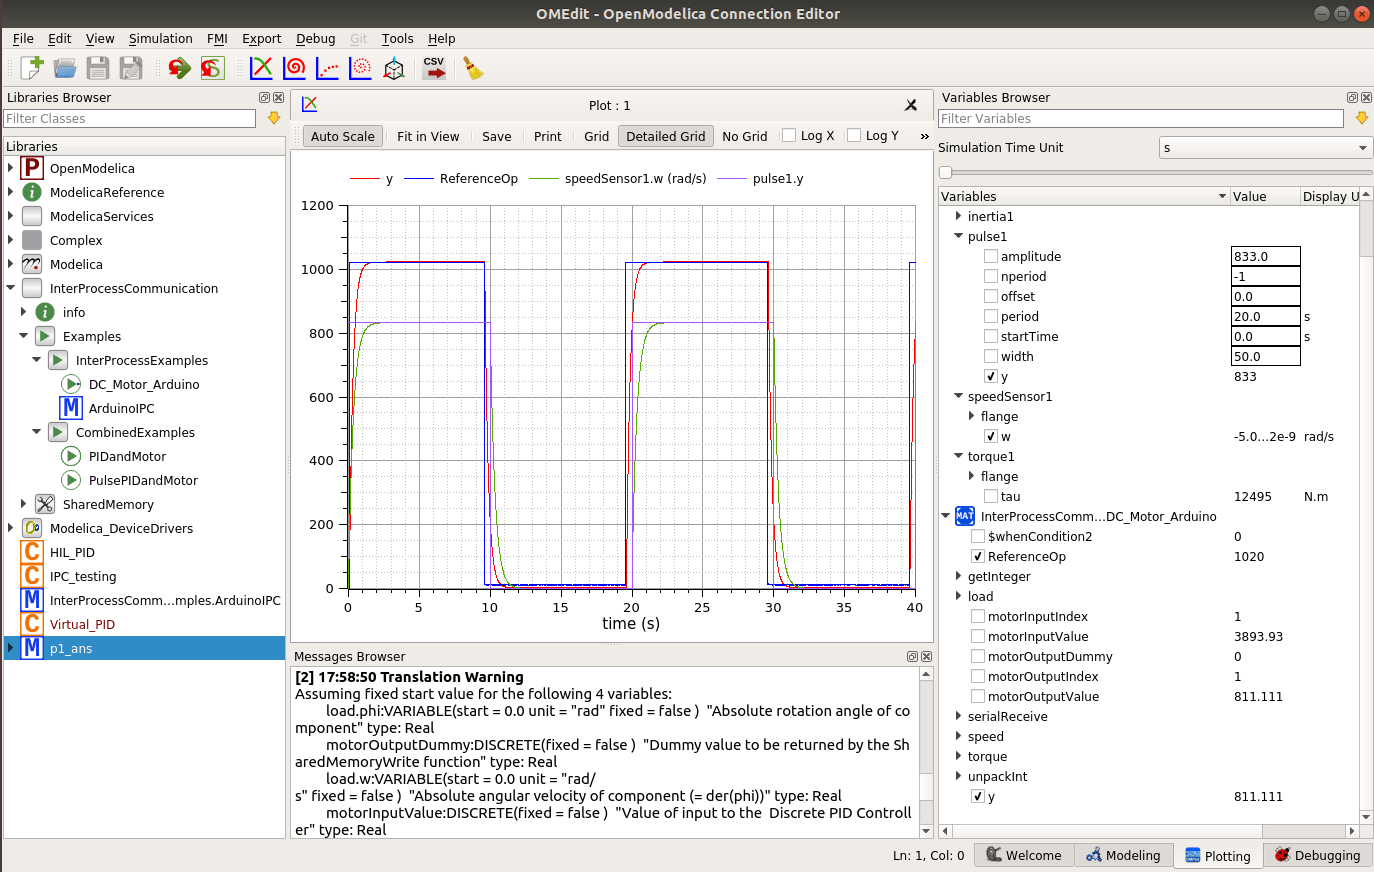
\includegraphics[scale=0.25]{Modelica_Output.png}
\end{document}